\documentclass[lettersize,journal]{IEEEtran}
\usepackage{amsmath,amsfonts}
\usepackage{algorithmic}
\usepackage{array}
\usepackage[caption=false,font=normalsize,labelfont=sf,textfont=sf]{subfig}
\usepackage{textcomp}
\usepackage{stfloats}
\usepackage{url}
\usepackage{verbatim}
\usepackage{graphicx}
\usepackage{booktabs}
\usepackage{multirow}  
\hyphenation{op-tical net-works semi-conduc-tor IEEE-Xplore}
\def\BibTeX{{\rm B\kern-.05em{\sc i\kern-.025em b}\kern-.08em
    T\kern-.1667em\lower.7ex\hbox{E}\kern-.125emX}}
\usepackage{balance}
% 设置超链接跳转
\usepackage[colorlinks,
linkcolor=blue,
anchorcolor=blue,
citecolor=blue]{hyperref} 
\usepackage{amsmath}

% 改变字体颜色
\usepackage{color,xcolor}
\usepackage{makecell}
\begin{document}
\title{UVDT: A Baseline Benchmark for Vehicle Digital Twins via LiDAR-Camera Fusion in Multi-Intersection Scenarios}
\author{IEEE Publication Technology Department

\thanks{Manuscript created October, 2020; This work was developed by the IEEE Publication Technology Department. This work is distributed under the \LaTeX \ Project Public License (LPPL) ( http://www.latex-project.org/ ) version 1.3. A copy of the LPPL, version 1.3, is included in the base \LaTeX \ documentation of all distributions of \LaTeX \ released 2003/12/01 or later. The opinions expressed here are entirely that of the author. No warranty is expressed or implied. User assumes all risk.}}

\markboth{Journal of \LaTeX\ Class Files,~Vol.~18, No.~9, September~2020}%
{How to Use the IEEEtran \LaTeX \ Templates}

\maketitle

\begin{abstract}
In this paper, we explore the application of digital twins in automated driving and propose Urban Vehicle Digital Twin(UVDT), which replicates the traffic flow by investigating four aspects: single-intersection multi-object tracking, multi-intersection multi-object tracking, trajectory inference and reduction, and twinning. 
The multi-object tracking performance is optimized by fusing radar detection and camera detection data to improve the accuracy and robustness of vehicle detection, which in turn solves the challenges posed by occlusion and view angle changes. 
Cross-scene vehicle re-recognition is improved by generating rich training data. 
The digital twin-based vehicle control method provides high-precision path planning and control for the autonomous driving system, ensuring accurate vehicle navigation in complex traffic scenarios. 
The experimental results show that UVDT can provide high-fidelity simulation scenarios for the testing and optimization of autonomous driving systems, which promotes the development of intelligent transportation systems and provides important support for the construction of future smart cities.
\end{abstract}

\begin{IEEEkeywords}
digital twins, automated driving, vehicle detection, multi-object tracking, trajectory reduction.
\end{IEEEkeywords}

\noindent \textbf{Code Availability:} The source code and datasets are available at \url{https://github.com/OpenHUTB/traffic_twin}.

\section{Introduction}

\IEEEPARstart{W}{ith} the rapid development of intelligent transportation, autonomous driving, and urban management, digital twin technology, as an important innovative tool, has gradually shown tremendous potential in various fields\cite{Alpher17}. 
A digital twin refers to the creation of a digital model corresponding to the real world through the real-time synchronization of data collected from the physical world and virtual models\cite{Alpher20c}. 
This technology can simulate, analyze, and optimize the real world in a virtual environment, thus providing support for decision-making\cite{Alpher21b}. 
In the field of autonomous driving, digital twin technology can accurately replicate factors such as traffic flow, road structure, and pedestrian behavior, providing a precise testing and training environment for the perception, planning, and control of autonomous driving systems\cite{Alpher24}\cite{Alpher20d}.

The focus of this research is to apply digital twin technology to the development and testing of autonomous driving systems to improve the interpretability and robustness of autonomous driving systems by replicating real traffic flow scenarios\cite{Alpher24b}.
By constructing high-precision digital twin models and combining reinforcement learning with simulation platforms, we are able to simulate complex driving scenarios and train and optimize autonomous driving algorithms\cite{Alpher22c}. 
At the same time, digital twin technology can provide smarter decision support for traffic management, promoting the development of smart city construction\cite{Alpher17b}.

\begin{figure}[t]
	\centering
	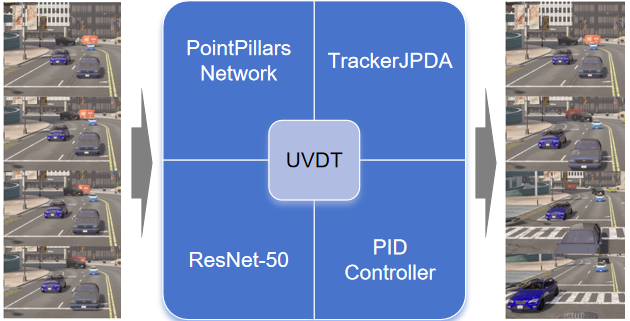
\includegraphics[width=\linewidth]{picture/picture1.png} 
	\caption{Overall Preview of Digital Twin through UVDT.} 
	\label{fig:example} 
\end{figure}

We primarily conducted research from four aspects: single-intersection multi-object tracking, multi-intersection multi-object tracking, trajectory inference and restoration, and digital twinning. 
Vehicle detection is a core perception task in autonomous driving systems, which usually relies on data from various sensors (such as lidar, cameras, and millimeter-wave radar) for object recognition and positioning. 
As a key input source for digital twin systems, the accuracy of vehicle detection directly affects the behavior modeling and scene restoration quality of traffic participants in virtual environments. 
In recent years, the application of deep learning technology has significantly improved the accuracy and robustness of vehicle detection, but it still cannot meet the challenges of vehicle occlusion and perspective changes in complex environments. Therefore, we use camera and radar fusion detection to improve the accuracy of vehicle detection, thereby improving the accuracy of vehicle tracking.

The most fatal problem in tracking vehicles in complex urban traffic environments is how to track the vehicle again after it is blocked. The current mainstream solution uses a multimodal sensor fusion framework: at the data level, feature complementarity of lidar, camera, and millimeter-wave radar is achieved through spatiotemporal alignment; at the decision level, an improved Kalman filter is used to weightedly fuse multi-source information. However, this solution has two major bottlenecks: sensor calibration error and appearance feature variation (such as illumination/perspective change). To this end, we use re-identification technology to re-track the vehicle. Even if the vehicle ID is switched, the skeleton models of different vehicles can still be effectively distinguished by appearance features, and the color changes of the same vehicle under different lighting conditions can be accurately identified, thereby providing a reliable identity association basis for vehicle tracking in multi-camera scenarios and ensuring the continuity and consistency of vehicle motion trajectories in complex environments\cite{Alpher23}.

In actual multi-target tracking applications, trajectory interruption and breakage are common technical challenges due to factors such as sensor detection distance limitations, target occlusion, and environmental noise. To address this problem, modern intelligent tracking systems usually use a hybrid method that combines kinematic models with deep learning to intelligently infer and complete lost trajectories to maintain spatiotemporal continuity. Some mainstream methods include trajectory prediction based on Kalman filtering or particle filtering, but they generally face challenges such as limited occlusion processing capabilities, insufficient nonlinear motion modeling, and the balance between computational efficiency and accuracy. To overcome these limitations, we use the efficient navigation algorithm framework in the CARLA simulation platform. This solution implements trajectory inference through the shortest path planning between two points. It is not only computationally efficient and not restricted by complex environments, but also has controllable errors due to the short distance.
Finally, by accurately simulating the vehicle's driving route and traffic behavior through integrated control algorithms, a complete autonomous driving system verification platform is formed, providing a reliable digital twin foundation for algorithm development and safety assessment\cite{Alpher24c}.

\section{Related Work}

We have summarized research work on different aspects of UVDT.

\textbf{Vehicle Detection.}
UVDT mainly uses LiDAR and cameras for vehicle object detection.
Several recent studies have explored the fusion of LiDAR and camera data for vehicle detection,demonstrating significant improvements in both accuracy and robustness. 
For instance, MVDNet (2018) utilizes a multi-view fusion approach, where LiDAR point clouds are projected to different views (such as bird’s-eye view and front view) and matched with camera images, combining depth information from LiDAR and texture information from the camera. 
This method improves detection performance, especially in complex environments\cite{Alpher22h}. 
Building on this, PointPillars introduces a fast encoder for LiDAR data, using a grid-based encoding approach that could potentially be integrated with camera data in future fusion methods to enhance detection speed and efficiency\cite{Alpher19}.
Another study combines LiDAR and camera data by feeding them into separate convolutional neural networks, where the features extracted from both modalities are fused to perform object detection\cite{Alpher20e}. 
This approach has shown significant improvements in detection performance, particularly in dynamic environments with occlusions or sparse LiDAR data.
Lastly, ST-MVDNet introduces a self-training framework using a teacher-student mutual learning mechanism, where the teacher network is trained on the fused LiDAR and camera data, while the student network is exposed to strong data augmentation simulating missing sensor modalities\cite{Alpher22f}. 

This approach enhances the model’s robustness against sensor failures by ensuring consistency between the teacher and student models, allowing the system to better handle missing or noisy data during inference.
These methods collectively highlight the importance of sensor fusion and advanced learning techniques in achieving robust and accurate vehicle detection, even in challenging conditions.
We use a combination of PointPillars-based 3D point cloud detection method and YOLOv4-based 2D image detection method for multimodal object detection.
These two deep learning methods have shown excellent detection performance in their respective fields.

\textbf{Multi-Object Tracking.}
Specker and his team proposed an online multi-camera multi-target tracking method (OCMCTrack), which dynamically optimizes cross-camera target association through an innovative Corrective Matching Cascade strategy, significantly improving tracking accuracy and ID consistency in complex scenarios while ensuring real-time processing\cite{Alpher24e}.
Shim and his team proposes a robust multi-target multi-camera vehicle tracking system designed for city-scale traffic management, addressing challenges like occlusion and cross-camera identity consistency by integrating spatial-temporal constraints and deep feature fusion to enable real-time vehicle monitoring and behavior analysis across urban camera networks\cite{Alpher21e}.
Most existing algorithms, with a few exceptions, can be seen as special cases of the multi-modal fusion problem. 
These methods organize the input data using a graph structure, where edges represent relationships between modalities, and nodes represent different targets or states. 
Algorithms that can be solved in polynomial time typically handle specific modalities or time-continuous edges, with some also utilizing maximum flow or matching algorithms. 
Methods that leverage global information (beyond just time continuity or modality constraints) can significantly improve performance, but they are usually NP-hard due to the involvement of combinatorial optimization. 
In some cases, marginal terms or local constraints are added to ensure completeness. 
To enhance model expressiveness, some studies have employed higher-order relations, although the gains diminish significantly as complexity increases. 
Joint optimization and iterative optimization strategies have also been widely used to improve performance.
We use Joint Integrated Probabilistic Data Association (JIPDA), which combines data from multiple sensors and optimizes probabilistic associations to effectively handle data uncertainty and missing information in target tracking, improving tracking accuracy and robustness in complex environments.


\textbf{Vehicle Reidentification.}
Bing and his team proposed a part-based regularization method, which enhances the accuracy of vehicle re-identification by detecting local parts of vehicles, such as lights and wheels\cite{Alpher19b}. 
Zheng and his colleagues introduced a large-scale vehicle re-identification dataset named VehicleNet and proposed a multi-task learning framework that combines vehicle re-identification and vehicle attribute recognition tasks, improving the model's generalization capability\cite{Alpher20f}. 
P and the research team proposed a dual-path model that integrates global and local features and incorporates an adaptive attention mechanism to enhance the accuracy of vehicle re-identification\cite{Alpher19c}.

The most advanced technologies in the field of vehicle re-identification currently include the combination of deep convolutional neural networks (CNN) for feature extraction and metric learning\cite{Alpher20g}, particularly with the integration of cross-view and cross-domain learning techniques, the use of Generative Adversarial Networks (GAN) for image enhancement\cite{Alpher21d}, and the fusion of multi-sensor data (such as cameras, radar, and LiDAR) to improve the model's robustness and accuracy in complex environments\cite{Alpher22g}.

Inspired by person Re-ID techniques for video sequences, we developed a retrained vehicle Re-ID network based on ResNet-50. 
The network has acquired comprehensive feature representations through large-scale image training, enabling effective vehicle re-identification performance.

\begin{figure*}[t]
	\centering
	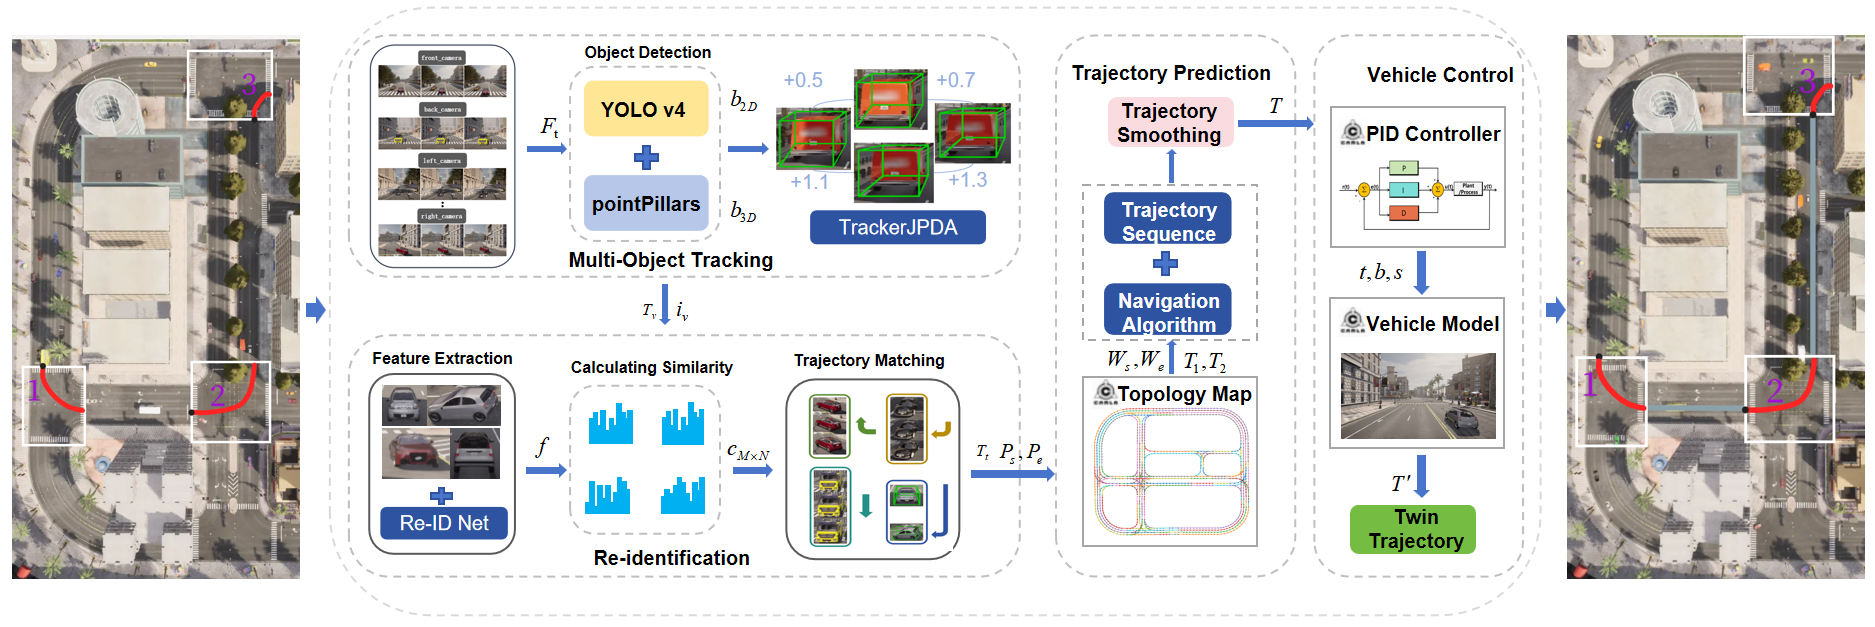
\includegraphics[width=\textwidth]{picture/picture2.png} 
	\caption{In the given scenario, synchronized cameras and LiDAR sensors detect vehicles, while the tracking system performs both single-intersection and multi-intersection multi-object tracking. The tracking data is subsequently utilized for trajectory reconstruction, ultimately enabling the creation of a digital twin that accurately replicates the traffic scenario.}
	\label{fig:2}
\end{figure*}

\textbf{Digital Twin.}
After obtaining the trajectory data of all tracked vehicles, we will use the vehicle control algorithm to reproduce the traffic flow in the simulation scenario.
Kaleb Ben Naveed et al. proposed a hierarchical reinforcement learning-based method for autonomous driving trajectory planning and control. 
By training a reinforcement learning agent in a simulation environment, this method optimizes the vehicle's control strategy according to environmental changes, achieving efficient trajectory planning and dynamic path adjustment.\cite{Alpher22}
R. Barea et al. proposed a deep reinforcement learning (DRL)-based control method, where an agent is trained in the CARLA simulation platform to autonomously learn and optimize the vehicle's control strategies (such as throttle, brake, and steering) to ensure safe and smooth driving.\cite{Alpher21}
We optimize the trajectories obtained from multi-object tracking using a trajectory smoothing algorithm, enabling the vehicle to turn more smoothly and drive more steadily (reducing bumps and sudden maneuvers) while ensuring precise adherence to the planned path at a lower computational cost. 
Subsequently, the PID controller is employed to control the vehicle, guiding it to follow the optimized trajectory and achieve final trajectory-tracking synchronization.


\section{Method}

\subsection{Problem Definition}

In UVDT, the vehicle detection and tracking system for single-intersection scenarios adopts a multimodal data fusion architecture.
As illustrated in Fig. \ref{fig:2}, the input source \(F_{t}\) integrates 3D point cloud data captured by LiDAR and synchronized RGB images from six calibrated cameras, achieving heterogeneous sensor data collaboration through spatiotemporal alignment.
The tracker generates the vehicle trajectory \(T_{v}\) of a single intersection and the image \(i_{v}\) of the corresponding vehicle through the detection bounding boxes \(b_{2D}\) and \(b_{3D}\) obtained by object detection algorithms.
For cross-intersection vehicle trajectories matching, we employ a re-identification network to extract appearance feature vectors \(f\), then compute their cosine similarity to produce a logical matching matrix \(C_{M \times N}\).
Vehicle trajectories exceeding a predefined similarity threshold are matched and output as \(T_{t}\).
The system subsequently feeds trajectory endpoints \((P_{s},P_{e})\) to a prediction framework that interpolates inter-intersection trajectories, ultimately producing complete vehicle trajectories \(T_{t}\). 
The controller calculates throttle\(t\), brake\(b\),and steering wheel \(s\) outputs from these trajectories to guide vehicle control, with the final executed trajectory denoted as \(T^\prime\).

\textbf{Vehicle Detection in Point Clouds.}
Based on the PointPillars network architecture, 3D vehicle detection in intersection scenes is implemented. Its input data is collected in real time through a 64-line laser radar (range measurement 200m/point cloud density 2.2M pts/s/scanning frequency 20Hz), and the 3D ground truth information of vehicles in the range is recorded simultaneously. The original dataset is divided into a training set and a test set in a 7:3 ratio. The training set is used to learn the mapping relationship from point cloud to 3D detection box, and the test set verifies the generalization ability of the model on unknown data.

A PointPillars network requires two inputs: pillar indices as a P-by-2 and pillar features as a P-by-N-by-K matrix. P is the number of pillars in the network, N is the number of points per pillar, and K is the feature dimension.
The network begins with a feature encoder, which is a simplified PointNet. It contains a series of convolution, batch-norm, and relu layers followed by a max pooling layer. A scatter layer at the end maps the extracted features into a 2-D space using the pillar indices.
Next, the network has a 2-D CNN backbone that consists of encoder-decoder blocks. Each encoder block consists of convolution, batch-norm, and relu layers to extract features at different spatial resolutions. Each decoder block consists of transpose convolution, batch-norm, and relu layers.
The network then concatenates output features at the end of each decoder block, and passes these features through six detection heads with convolutional and sigmoid layers to predict occupancy, location, size, angle, heading, and class.

\textbf{ReID.}
Re-identification is a crucial component of multi-object tracking, aimed at addressing the issue of temporary object occlusion in videos. 
In real-world scenarios, tracked objects may be temporarily obscured by other objects or move out of the camera's field of view, making consistent tracking challenging. 
These objects may also exhibit variations in pose, orientation, and lighting conditions between frames. 
In such complex scenarios, when an object reappears in a new video frame, the tracker often fails to re-identify the object. 
Consequently, the tracker begins to treat the object as a new entity. 
This misidentification leads to errors and inconsistencies in object tracking.

ReID aims to resolve this issue by matching the features of an object in a new frame with those of previously tracked objects, thereby identifying the same object even if it appears in a different location or orientation, or under varying lighting conditions compared to the previous frame. 
This approach ensures that the tracker can maintain consistent tracking information for a given object\cite{Alpher24d}.


\subsection{Single Intersection Multi-Object Tracking}

We fuse detections from our lidar and camera at a single intersection and use the tracker JDPA object to track the target.

\textbf{Single Detection Class Probability Update.}
First, consider the class information association between one detection and one track. 
Assume the confusion matrix of the detection is \(C=\left[c_{i j}\right]\), where \(c_{i j}\) denotes the likelihood that the classifier outputs the classification as \(j\) if the truth class of the target is \(i\).
Here, \(i,j = 1,…, N\), and \(N\) is the total number of possible classes.
At time \(k-1\), the probability that the trajectory is classified as \(i\) is \(\mu_{i}(k-1)\).
If the tracker associates the detection to the track at time \(k\), then the updated value of \(\mu_{i}\) using Bayes' theorem is
\begin{align}
	\mu(k) & = \frac{c_{j} \otimes [ \mu_1(k-1), \ldots, \mu_N(k-1) ]^T}{c_{j}^{T} [ \mu_1(k-1), \ldots, \mu_N(k-1) ]^T}
\end{align}
where \(c_{j}\) is the \(j\)-th column of the confusion matrix and \(\otimes\) represents element-wise multiplication. 
This equation represents the updated class probability of a track if the track is associated with the detection of classification \(j\).

\textbf{Mixed Association Likelihood in Cluster.}
The tracker performs gating and clustering by using only the kinematic information between detections and tracks. 
After that, in each cluster, the tracker calculates the mixed likelihood of association between a detection \(m\) and a track \(t\) as:
\begin{align}
	\Lambda(m, t) & = \Lambda_{k}^{1-\alpha}(m, t) \Lambda_{c}^{\alpha}(m, t)
\end{align}
where \(\alpha\) represents Weight factor of class likelihood; \(\Lambda_{k}\) represents Likelihood of assigning a detection to a track based on the kinematic states; \(\Lambda_{c}\) represents Likelihood of assigning a classified detection to a track based on the class information.
\begin{align}
	\Lambda_{c}(m, t) = \left\{\begin{array}{ll}
		c_{j}^{T}\left[\mathbb{I}_t \mu(k-1)+\mathbb{I}_{t = 0} \mu^{0}\right] & \text { if } m>0 \\
		1 & \text { if } m = 0
	\end{array}\right.
\end{align}
The hybrid association likelihood function achieves multi-scenario adaptive matching through a triple mechanism: for valid associated targets (\(m>0\) and \(t>0\)), the system corrects the trajectory category probability distribution \(\mu(k-1)\) in real time through Bayesian updating, and uses the confusion matrix column vector \(c_j\) of the detection m corresponding to category \(j\) to calculate the matching degree, thereby dynamically adapting to changes in target categories; for new targets (\(m>0\) and \(t=0\)), the prior distribution \(\mu^{0}\) based on the statistical characteristics of the data set is used for initialization to effectively solve the cold start problem; for unmatched trajectories (\(m=0\)), a fixed value of 1 is returned to avoid false termination caused by sensor noise. The design achieves the optimal fusion of kinematics and category information through the \(\alpha\) parameter, significantly improving the tracking robustness in complex scenarios while ensuring real-time performance.

\textbf{Update Track Class Probability.}
Suppose the marginal probabilities of \(M\) detections assigned to a track in the cluster are \(\left(\beta_{0}, \beta_{1}, \ldots, \beta_{M}\right)\), where \(\beta_{0}\) is the marginal probability that no measurements is associated with the track. 
Then the tracker updates the class probability of the track as
\begin{align}
	\mu_{k} & = \left(\sum_{m = 1}^{M} \beta_{m} \frac{c_{j(m)} \otimes \mu(k-1)}{c_{j(m)}^{T} \mu(k-1)}\right)+\beta_{0} \mu(k-1)
\end{align}
where \(c_{j}(m)\) is the class probability vector of detection \(m\), \(\otimes\) represents element-wise multiplication, \(\mu(k-1)\) is the class probability vector of the track in the \(k-1\) step, and \(\mu(k)\) is the class probability vector of the track in the \(k\) step.

The tracker updates the class properties of tracks cluster by cluster.

\textbf{Process.}

In this process, we employ a tracker to handle the 2D and 3D bounding boxes obtained from target detection, along with their corresponding timestamps. 
The tracker utilizes a soft assignment strategy, allowing each trajectory to integrate contributions from multiple detection results. 
Its responsibilities include trajectory initialization, confirmation, correction, prediction (including prediction in a coasting state without active motion), and deletion. 
For each trajectory, the tracker estimates its state vector and the covariance matrix of the state estimation error. 
It ensures that every detection is assigned to at least one trajectory; if a detection cannot be matched to any existing trajectory, the tracker creates a new one.

Newly generated trajectories are initially in a tentative state. 
When a tentative trajectory accumulates a sufficient number of detection assignments, its status transitions to confirmed. 
If the detections themselves already carry explicit classification information (i.e., the returned trajectory data contains non-zero fields), the corresponding trajectory is immediately confirmed as valid. 
Once a trajectory is confirmed, the tracker recognizes it as representing a real physical object. 
However, if a trajectory fails to receive any detection assignments within a predefined number of update cycles, it will be deleted.

Through this process, we are ultimately able to obtain the trajectories of vehicles within the intersection.

\textbf{Reference System.}

We placed an imaginary ego-vehicle in the center of the intersection, which serves as a reference system, as shown in Fig. \ref{fig:3}. 
For multi-object tracking we input not only the detection frame, but also the position of the camera and radar relative to the self-vehicle, as well as the position of the ego-vehicle. 
The position coordinates of the self-vehicle in the experiment were always O(0,0,0), i.e. stationary. 
Tracking initially generates trajectory coordinates \(\text P_1\) relative to the LiDAR, which we also fit to the world coordinates \(\text P_2\) in Carla.
\begin{figure}[t]
	\centering
	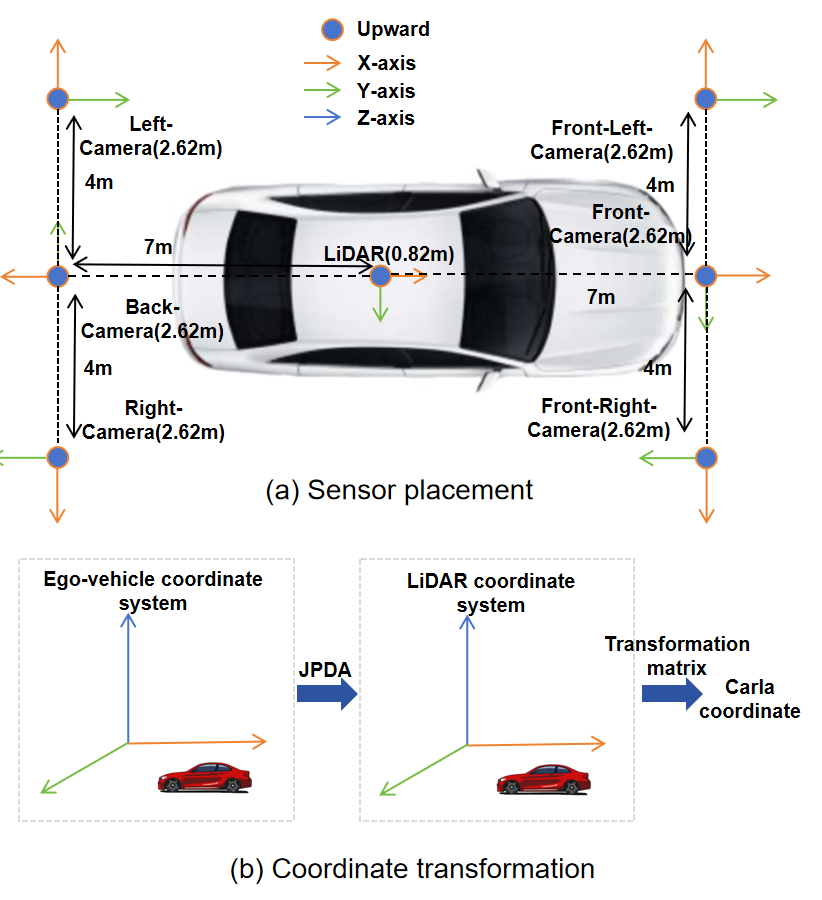
\includegraphics[width=\linewidth]{picture/picture3.png} 
	\caption{Sensor configuration and coordinate transformation process: (a) Multi-sensor arrangement on the ego vehicle, including 6 cameras (2.62 meters upward offset) and 1 lidar (0.82 meters upward offset); (b) Coordinate transformation process from the ego vehicle system (left) to the lidar coordinate system (right) through JPDA, and finally converted to the CARLA world coordinate system through the transformation matrix. All distance measurements are in meters.} 
	\label{fig:3} 
\end{figure}

\subsection{Multi Intersection and Multi-Object Tracking}

In the Town10 scene of the CARLA simulation platform, we configure a differentiated blueprint for each experimental vehicle, so that it strictly follows the preset path from a fixed starting point to a specified end point, and build a fully controllable and highly reproducible dynamic traffic scene.
To achieve all-round data collection, we deploy RGB cameras and semantic segmentation cameras at the front and rear positions of each experimental vehicle, respectively, and use a multi-view synchronous acquisition system to capture the continuous changes in the vehicle's appearance features and spatial posture in real time, and finally generated dynamic ground truth and image sequences with precise spatiotemporal alignment characteristics.

Subsequently, the vehicle images of the front and rear views are cropped based on ground truth and the front and rear view images of the same vehicle are combined to form a dataset of that vehicle, to which the vehicle images of the occluded views are added to form the final dataset.
Before training the re-identification network, the images were reshaped to a size of 224\(\times\)224, of which 90\% were used as training sets and the rest as validation sets.

Finally, the images of vehicles tracked at intersections 1 and 2 are matched with the trained re-identification network.
In other words, the vehicle tracked at the previous intersection is the object that needs to be re-identified, and it will be recognized at the next intersection, allowing the trajectories corresponding to the two vehicles to be integrated.

For matching vehicle trajectories between intersections, we use a re-recognition network to extract features from the vehicle images and then compute the cosine similarity of these two features.
If Intersection 1 has M vehicles and Intersection 2 has N vehicles, a matrix of size M×N is generated. 
If the similarity exceeds a certain threshold, the two vehicles are considered to be the same vehicle.

\textbf{ResNet-50.}
ResNet-50 primarily consists of five main components: an initial convolutional layer, a max-pooling layer, four stages of residual blocks, a global average pooling layer, and a fully connected layer, totaling 50 layers (including convolutional layers, pooling layers, and fully connected layers). 
Among these, the four stages of residual blocks are the core of ResNet-50. 
The first residual block in each stage performs downsampling on the size of the feature maps, while the subsequent residual blocks maintain the same feature map size.

ResNet-50 employs a residual block structure known as Bottleneck, which aims to reduce computational complexity. 
Each residual block consists of the following layers:

\(\bullet\) 1\(\times\)1 Convolutional Layer: Used for dimensionality reduction, decreasing the number of channels.

\(\bullet\) 3\(\times\)3 Convolutional Layer: Used for extracting spatial features.

\(\bullet\) 1\(\times\)1 Convolutional Layer: Used for dimensionality increase, restoring the number of channels.

\(\bullet\) Residual Connection: The input is directly added to the output of the 1\(\times\)1 convolutional layer. 
If the number of channels or the size of the input and output do not match, a 1\(\times\)1 convolution is applied to adjust the input.

Each convolutional layer is followed by batch normalization and a ReLU activation function.

\subsection{Trajectory Inference and Reconstruction}

\textbf{Inference of Trajectories in Unknown Regions.}
Upon completing the tracking of all vehicle trajectories, we chronologically sort the trajectory of each vehicle and select the last waypoint of the same vehicle at the previous intersection along with the first waypoint at the next intersection as the starting and ending points of the unknown region. 
These two waypoints are then fed into the navigation algorithm module, which subsequently computes the trajectory between them.

In the Carla simulation environment, vehicle trajectory planning is achieved by utilizing the A* algorithm to search for the shortest path within the graph structure constructed from the topological map. 
The A* algorithm evaluates the comprehensive cost of nodes and, at each step, selects the node with the lowest comprehensive cost for expansion, thereby effectively guiding the current node \(p_{n}\) to search for the target node \(p_{g}\).
The core of this algorithm lies in the evaluation function 
\begin{align}
	f(n) = \sum_{k = 1}^{n} \frac{d_{k} \cdot\left(1+\alpha \phi_{k}\right)}{1 + \frac{\gamma}{\kappa_k + \epsilon}}+\left\|\left[\begin{array}{c}
		p_{n}-p_{g} \\
		\sqrt{\lambda}\left(l_{n}-l_{g}\right)
	\end{array}\right]\right\|_{2}
\end{align}
Its purpose is to calculate the actual cost from the starting node to the current node and the estimated cost from the current node to the target node. 
In the process of exploring the shortest path using the A* algorithm, if there are edges with a weight of 0 in the graph structure, it may cause the vehicle to change lanes too frequently in a very short time, which contradicts the normal driving logic. 
To alleviate this phenomenon, we introduced a lane change penalty mechanism in path planning. Specifically, when the current lane \(l_{n}\) is inconsistent with the target lane \(l_{g}\), the calculation cost will be increased to ensure that the distance calculation between nodes is not only based on the spatial distance, but also takes into account the frequency of lane changes. Not only that, we also added a road type penalty \(\phi_{k}\) and a curvature penalty \(\kappa_k\). When planning the route globally, the vehicle prefers the main road and the road with smaller curves. 
Among them, \(\alpha\) represents the road attribute weight, \(\gamma\) controls the curvature penalty intensity, \(\lambda\) is the lane matching weight, and \(\epsilon\) is used as a regularization parameter to ensure numerical stability.


\textbf{All Trajectory Restoration.}
Through the aforementioned algorithmic framework, we are able to obtain vehicle trajectories in unknown regions. 
Simultaneously, we have also acquired vehicle trajectories at intersections using the JPDA tracker. 
At this point, we only need to concatenate all trajectories of the same vehicle in chronological order and place them into a new collection, thereby obtaining the complete trajectory of that vehicle. 
This method can be represented as: 
\begin{align}
	S(t) = \bigcup_{i=1}^{N} \Bigl( T_i(t) \cup f\Bigl( \lim_{\!t \to t_i^+} T_i(t), \lim_{\!t \to t_{i+1}^-} T_{i+1}(t) \Bigr) \Bigr)
\end{align}
where \(S\) is the trajectory collection, \(T_i(t)\) represents the previous trajectory. 
The limits \(\lim_{t \to t_i^+} T_i(t)\) and \(\lim_{t \to t_{i+1}^+} T_{i+1}(t)\) correspond to the end waypoint of the \(i\)-th trajectory and the start waypoint of the \((i+1)\)-th trajectory, respectively.
As demonstrated in Fig. \ref{fig:5}, we can derive the complete vehicle trajectory collection, effectively reconstructing the trajectories of all vehicles.
\begin{figure}[t]
	\centering
	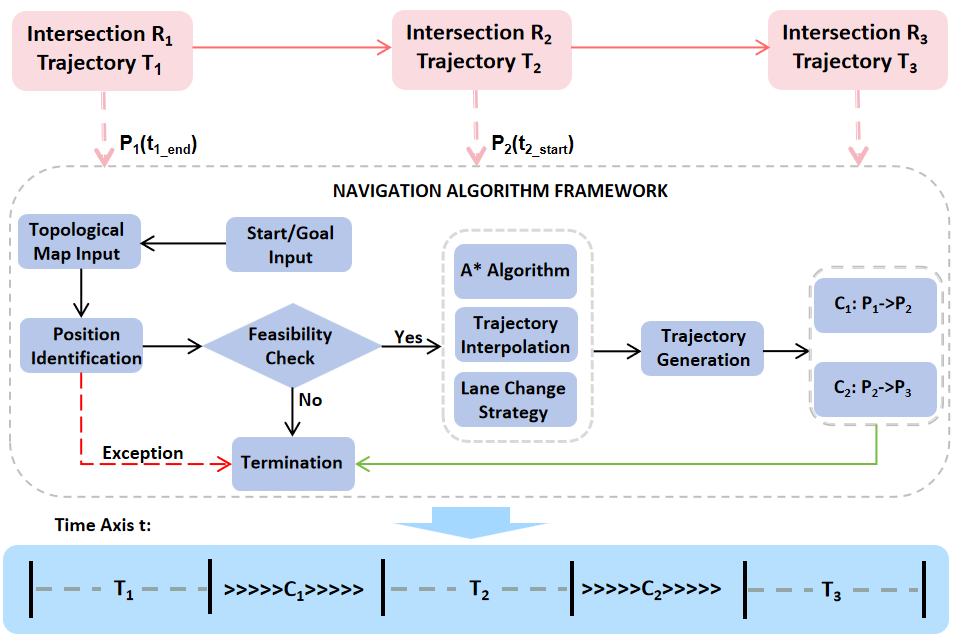
\includegraphics[width=\linewidth]{picture/picture5.png} 
	\caption{Trajectory restoration diagram, showing how to generate predicted trajectories between intersections from multi-target tracking trajectories and then obtain the complete vehicle trajectory.} 
	\label{fig:5} 
\end{figure}

\subsection{Twin of Trajectory}

Through the previous steps, we have obtained the trajectories of all vehicles. 
Here, we will further optimize these trajectories using a trajectory smoothing algorithm, and then employ a PID controller to control the vehicles, ensuring they follow the optimized trajectories\cite{Alpher22d}. 

A trajectory smoothing method based on linear interpolation is adopted in this work.
Given the original trajectory point set \(W = \{w_1,w_2 ,…,w_n\}\), where \(w_i \in R^2\) represents the coordinates of the \(i\)-th track point, the smoothed track \(\widetilde{W}\) is generated by:
\begin{align}
	\widetilde{W} = \bigcup_{i = 1}^{n-1} \left( w_i \cup \left\{ w_i + k\delta \cdot \frac{w_{i+1} - w_i}{d_i} \ \middle|\ k \in \mathbb{N}^+\right\} \right)
\end{align}
Precise control of trajectory density is achieved through a step size parameter \(\delta\) in this method, which maintains strict adherence to the original trajectory geometry and ensures all interpolation points are positioned on line segments connecting adjacent original waypoints.
Specifically, for any adjacent waypoint pair, the algorithm uniformly inserts new waypoints on its connection line. The number of insertion points is dynamically determined by the ratio of distance \(d_i\) to step \(\delta\), and the constraint \(k\delta < d_i\) is satisfied, thereby ensuring the adaptive matching of the interpolation density and the local geometric features of the trajectory.
It is worth noting that the current method assumes that the input waypoints are all on the real trajectory, and for the filtering of possible external or noise points, an additional robust processing mechanism is needed, which will be an important direction for future research.

The PID controller consists of three main components: Proportional control (P), Integral control (I), and Derivative control (D). Each component serves a specific purpose, enabling the regulation of different aspects of the system.

\begin{align}
	u = K_p e + K_i \int \left( e - \frac{\text{sat}(u)-u}{K_p} \right) dt + K_d \dot{e}
\end{align}
This study proposes an improved PID control algorithm, whose control output \(u\) consists of proportional term, anti-saturation integral term, and differential term, where \(K_p\), \(K_i\) and \(K_d\) are proportional gain, integral gain and differential gain respectively.
The algorithm achieves rapid error response through the proportional term, eliminates steady-state errors using the integral term, and suppresses the error change rate through the differential term.
Experimental studies have shown that traditional PID control has an integral saturation phenomenon in the vehicle steering system, resulting in random extreme deflections of the steering wheel (±1 rad).
To this end, this algorithm introduces a compensation term, and the saturation function sat(u) limits the controller output \(u\) to a preset interval [\(u_{min}\), \(u_{max}\)].
When the control output reaches the saturation limit, the integral accumulation rate is automatically adjusted, which effectively solves the integral saturation problem.
In addition, \(\dot{e}\) represents the rate of change of the error over time.

The tuning process of the PID controller is as follows:  
1. Calculate the error \(e\) between the target value (setpoint) and the current system output in real time.  
2. Compute the proportional action based on the current error, the integral action based on historical errors, and the derivative action based on the rate of change of the error.  
3. Sum the results of the proportional, integral, and derivative components to obtain the final control output, which is then applied to the system (for example, adjusting the vehicle's acceleration or direction). 
4. The system adjusts based on the control output, changing its state (for example, speed, position, etc.). 
The controller continues to monitor the system state, updates the error in real time, and repeats the above steps until the system stabilizes near the target value.


\subsection{Evaluation}

We employed three evaluation metrics.

\textbf{Multiple Object Tracking Accuracy.}
Single-camera, multi-object tracking performance is typically measured by the Multiple Object Tracking Accuracy \((MOTA)\)\cite{Alpher23b}.
We use an improved evaluation metric Robust Multi-Object Tracking Accuracy \((RMOTA)\) based on sliding window median statistics, which aims to enhance the robustness of traditional \(MOTA\) to short-term occlusion and ID switching.
The tracking sequence is divided into \(W\) time windows, and each window independently calculates the local \(MOTA\) score to avoid the serious error of a single frame affecting the overall evaluation.
In addition, the penalty for identity mismatching is amplified by the coefficient \(\alpha\) to reflect the key impact of ID continuity on tracking quality.
\begin{align}
	RMOTA = \underset{i=1}{\overset{W}{\mathrm{median}}} \left(1 - \frac{FN^{(i)} + FP^{(i)} + \alpha M^{(i)}}{T^{(i)}}\right) 
\end{align}
Among them,
\(FN^{(i)}\) (False Negatives) represents the number of missed detections in the \(i\)-th window, which means targets that truly exist but were not detected.
\(FP^{(i)}\) (False Positives) represents the number of false detections in the \(i\)-th window, which means targets that were detected but do not actually exist.
\(M^{(i)}\) (Mismatches) represents the number of identity mismatches in the \(i\)-th window, which means cases where the tracking ID of a target was incorrectly assigned during the tracking process.
\(T^{(i)}\) (Total number of true detections) represents the total number of true detections in the \(i\)-th window, which means the number of targets correctly detected across all frames.

The metric ranges from 0 to 1, with higher values indicating better tracking performance. 
A perfect score of 1 represents flawless tracking with zero missed detections, false alarms, or identity mismatches, while 0 indicates complete tracking failure.

\textbf{Cross-Sensor Tracking Accuracy.}
Multi-camera object tracking accuracy \((MCTA)\)\cite{Alpher23b} condenses all aspects of system performance into a metric that measures cross-camera tracking.
On this basis, this paper proposes an interpretable multi-camera object tracking accuracy \((IMCTA)\), which is defined as follows:
\begin{align}
	IMCTA = {\frac{2PR}{P + R}}_{\text{}} \times \prod_{k \in \{w, h\}} \left(1 - \frac{M_k + \lambda E_k^{\text{ID}}}{T_k}\right)
\end{align}
by decomposing the cross-camera error into missing association \(M_k\) and ID switching \(E_k^{\text{ID}}\), accurate diagnosis of system defects is achieved.
Among them,
\(P\) represents the proportion of correct matches (correctly identifying and tracking targets) across all cameras.  
\(R\) represents the recall rate, which is the proportion of all true targets that are correctly tracked.  
\(\lambda\) is the penalty coefficient for ID switching error and \(T^{k}\) represents the total number of potential correct associations in the \(k\)-th dimension, but the association thresholds for different dimensions are different.

Compared with \(MCTA\), \(IMCTA\) intuitively demonstrates the independent evaluation and synergy of detection capability and cross-camera association capability, transforming complex cross-camera evaluation into a transparent framework that is quantifiable, adjustable, and diagnosable. 
The higher the value, the better the performance of the multi-camera tracking system.

\textbf{Twin Accuracy.}
In the twin experimental evaluation, we verify the effectiveness of the system by comparing the comprehensive performance of the following three key trajectories: (1) the actual trajectory of the vehicle, (2) the observed trajectory reconstructed based on the multi-target tracking algorithm, and (3) the expected trajectory generated by the control system.
This study uses trajectory overlap ratio (TOR) for comprehensive evaluation, which quantifies both the shape similarity of the trajectory and the spatiotemporal consistency of the waypoints.
\begin{align}
	TOR & = \left(1 - \frac{D_{dtw}}{D_{max}}\right) \times \Lambda(t)
\end{align}
Among them, the shape similarity term is calculated based on the ratio of the dynamic time warping distance \(D_{dtw}\) to the maximum scale distance \(D_{max}\), reflecting the overall geometric difference of the trajectory, while the spatial alignment term \(\Lambda(\tau)\) evaluates the static matching accuracy of the waypoint through the position offset penalty.
This evaluation mechanism can not only capture the morphological differences of macroscopic paths, but also characterize the spatiotemporal consistency of discrete waypoints at the micro level, providing a multi-dimensional quantitative basis for the trajectory consistency of the digital twin system.
\begin{align}
	D_{dtw} = \min_{\pi \in P} \sqrt{\sum_{(i,j)\in\pi} \|p_i - q_j\|^2}
\end{align}
\begin{align}
	D_{max} = \max_{i,j} \|p_i - q_j\| \cdot \max(n,m)
\end{align}
\(D_{dtw}\) compares the similarity of non-aligned sequences through a dynamic curved path \(\pi\), and finds the matching solution that minimizes the cumulative distance from all possible path sets \(P\), while \(D_{max}\) quantifies the spatial deviation of the two trajectories in the worst case and normalizes it by the trajectory length. Among them, \(p_{i}\) and \(p_{j}\) represent the matching point pairs of the two trajectories, and \(m\) and \(n\) are the lengths of the two trajectories respectively.

\begin{align}
	\Lambda(\tau) = \frac{1}{n} \sum_{k=1}^{n} \mathbb{I}\left(\left\|p_{\pi_{1}(k)}-q_{\pi_{2}(k)}\right\| \leq \tau\right)
\end{align}
The trajectory we finally get is the coordinates of Carla, which means that the trajectory is actually discrete.
Therefore, calculating the positional relationship between waypoints is very important to reflect the overlap between two trajectories.
\(\Lambda(\tau)\) counts the proportion of matching points in the two trajectories whose distance is less than the threshold \(\tau\) to reflect the overlap accuracy of the two trajectories within the allowable error range.
where \(p_{\pi_{1}(k)}\) and \(q_{\pi_{2}(k)}\) represent the three-dimensional coordinates of the \(\pi_{1}(k)\)th point of trajectory 1 and the \(\pi_{2}(k)\)th point of trajectory 2, respectively, and \(\mathbb{I}(\cdot)\) is the indicator function (which takes the value of 1 when the Euclidean distance between two points does not exceed the threshold \(\tau\), otherwise it takes the value of 0).


\section{Experiments}

\subsection{Preparation}

\begin{table*}[t]
	\centering
	\caption{MULTI-OBJECTIVE TRACKING EVALUATION}
	\label{tab:2}
	\small
	\begin{tabular}{@{}l@{\hspace{1em}}c@{\hspace{0.5em}}*{10}{r}@{}}
		\toprule
		\textbf{Scene} & \textbf{Int.} & \textbf{Rcll} & \textbf{Prcn} & \textbf{FTR} & \textbf{FP} & \textbf{FN} & \textbf{IDS} & \textbf{MT} & \textbf{ML} & \textbf{RMOTA} & \textbf{RMOTP} \\
		\midrule
		\multirow{5}{*}{\shortstack[l]{Town01 \\ (16 int., flat roads, \\ sparsely populated \\ buildings)}} 
		& 1 & 30.1025 & 59.9258 & 0.5106 & 216 & 750 & 18 & 0.0000 & 37.5000 & 8.2945 & 79.9222\\
		& 2 & 64.8065 & 61.5385 & 1.0297 & 450 & 391 & 21 & 55.5556 & 33.3333 & 22.4122 & 86.7746\\
		& 3 & 63.2135 & 45.4407 & 1.1887 & 359 & 174 & 15 & 0.0000 & 25.0000 & -15.8562 & 86.9053\\
		& 4 & 65.8206 & 96.7662 & 0.0369 & 13 & 202 & 20 & 40.0000 & 20.0000 & 60.2369 & 89.0919\\
		& 5 & 41.4035 & 90.0763 & 0.0580 & 13 & 167 & 10 & 50.0000 & 0.0000 & 33.3333 & 88.2471\\
		\midrule
		\multirow{5}{*}{\shortstack[l]{Town10 \\ (7 int., high-density, \\ including steep slo- \\ pes)}} 
		& 1 & 30.6653 & 59.7166 & 0.7960 & 398 & 1334 & 28 & 8.3333 & 50.0000 & 8.5239 & 84.6488\\
		& 2 & 56.4410 & 70.6095 & 1.1380 & 569 & 1055 & 29 & 13.3333 & 26.6667 & 31.7506 & 81.0920\\
		& 3 & 51.9805 & 75.6714 & 0.6160 & 308 & 885 & 17 & 14.2857 & 35.7143 & 34.3462 & 84.2826\\
		& 4 & 52.1930 & 86.1427 & 0.2680 & 134 & 763 & 50 & 27.2727 & 36.3636 & 40.6642 & 88.6035\\
		& 5 & 45.4243 & 62.2719 & 1.6540 & 827 & 1640 & 35 & 12.5000 & 37.5000 & 16.7388 & 86.0825\\
		\bottomrule
	\end{tabular}
\end{table*}

\textbf{Simulation Environment.}
We conducted simulation experiments in Carla, whose advantage lies in its provision of a highly realistic virtual environment capable of accurately simulating complex traffic scenarios and diverse driving conditions. 
Carla supports flexible sensor configurations, such as cameras and LiDAR, facilitating multimodal data acquisition and fusion experiments\cite{Alpher22e}. 
We conducted relevant experiments in the Town10 and Town01 scenes in Carla.
The complex urban structure and dense traffic flow of Town10 can simulate highly dynamic real traffic environments, while the simple layout and clear rules of Town1 make it easy to construct controlled experimental scenarios.
This scene diversity can effectively verify the generalization ability of the model under different traffic conditions and provide a reliable basis for actual road deployment.

\textbf{Data Collection.}
In CARLA's Town10 scenario, a single intersection location is selected, with a LiDAR placed at the center and six cameras arranged around it to achieve 360-degree omnidirectional perception coverage. 
This setup allows for the acquisition of rich point cloud data and image information, making it suitable for target recognition and tracking in complex traffic environments. 
The same 64-line LiDAR configuration as that used for collecting PointPillars network training data is used, and a wide-angle camera with a resolution of 1920\(\times\)1080 pixels and a field of view of 90° is deployed simultaneously to achieve multimodal collection of point cloud and high-definition image data.
The collected data includes point cloud data from the LiDAR and image data from the cameras. 
The radar data is saved as MAT files with timestamps, while the camera data is saved as images for each frame in six directions. 
The data structure follows the storage format of the Panda dataset, making the data more standardized for subsequent processing and fusion\cite{Alpher21c}. 
Each frame of data synchronously collects six-directional camera images and LiDAR data containing point clouds, timestamps, and the coordinates of the sensor relative to the ego-vehicle.

\begin{figure}[t]
	\centering
	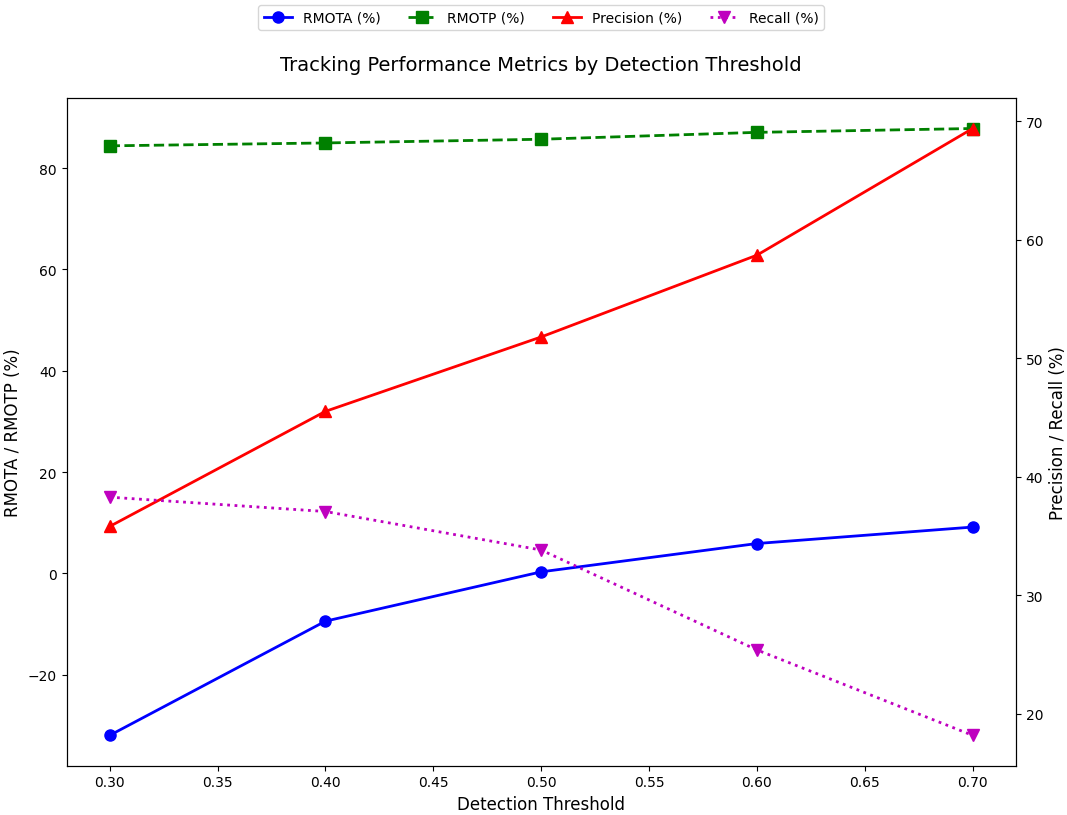
\includegraphics[width=\linewidth]{picture/picture6.png} 
	\caption{Analysis of the impact of point cloud detection threshold on multi-object tracking performance. Experiments show that the accuracy and threshold of vehicle detection are the key factors affecting tracking performance.} 
	\label{fig:6} 
\end{figure}

\begin{figure}[t]
	\centering
	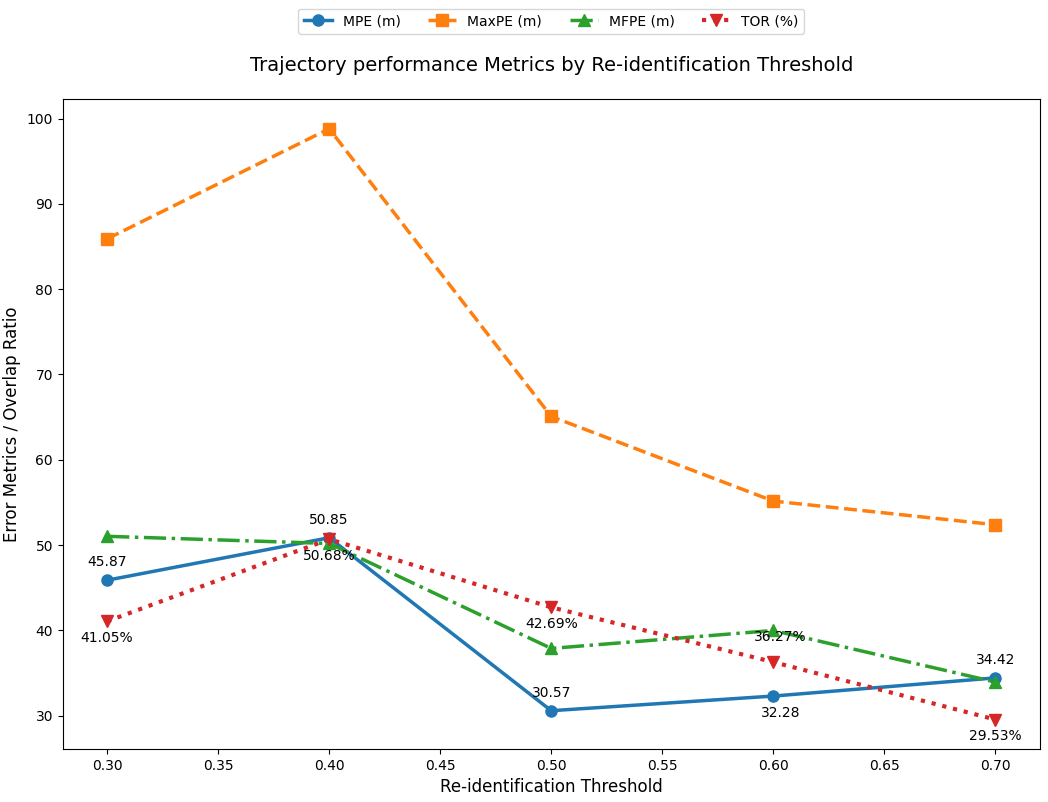
\includegraphics[width=\linewidth]{picture/picture7.png} 
	\caption{Comparative analysis of vehicle re-identification threshold effects on trajectory matching accuracy, illustrating the relationship between threshold values and the alignment degree between tracked trajectories and ground truth trajectories in urban traffic scenarios.} 
	\label{fig:7} 
\end{figure}

\subsection{Experimental Effect}

\textbf{Multi-Object Tracking.}
Table. \ref{tab:2} presents the multi-object tracking performance metrics across different scenarios (Town01 and Town10) and intersections (Intersection 1-5). 
The data reveals significant variations in performance across different intersections. 
In Town01, Intersection 4 shows better performance in terms of Recall (65.8206) and Precision (96.7662), while Intersection 3 has a higher False Track Ratio (1.1887), indicating a greater proportion of incorrect tracking. 
In Town10, Intersection 4 also demonstrates relatively high Recall (52.1930) and Precision (86.1427), but Intersection 5 has significantly higher False Positives (827) and False Negatives (1640) compared to other intersections, suggesting a higher number of misidentified and missed targets.

Identity Switches (IDS) are notably higher in Intersection 4 of both Town01 and Town10, with values of 20 and 50 respectively, indicating more frequent target identity switches at these intersections. 
The Mostly Tracked (MT) and Mostly Lost (ML) metrics show that Intersection 2 in Town01 has a higher MT (55.5556), while Intersection 1 in Town10 has a higher ML (50), reflecting significant differences in tracking stability across these intersections.

Overall, the tracking performance varies significantly across intersections. Intersection 4 in Town01 achieves high scores for both metrics (\(RMOTA\): 60.2369; \(RMOTP\): 89.0919), while Intersection 5 in Town10 shows notably lower accuracy (\(RMOTA\): 16.7388), indicating weaker tracking reliability.
However, detection accuracy is also affected by the number of vehicles passing through the intersection, and the system accuracy improves significantly in low traffic conditions.
These data highlight the performance variations of the multi-object tracking system across different scenarios and intersections, providing valuable insights for further optimization.

\textbf{Twin.}
The performance of the digital twin is primarily reflected by two sets of metrics: trajectory coincidence and control error (as shown in Table. \ref{tab:3} and \ref{tab:4}). 
These two tables compare the performance evaluation metrics of the digital twin in two scenarios, Town01 and Town10. 
The TOR in Town01 is significantly higher than that in Town10 in the comparison of the tracking trajectory with the digital twin trajectory (TR-DT), indicating that it has a superior path tracking ability, which may be due to the simpler environment or the more stable control algorithm.
However, for the comparison between the tracked trajectory and ground truth (TR-GT), it is higher in Town10, probably because our point cloud dataset was collected in Town10 and is more suitable for vehicle detection in this scenario.
In terms of mean position error (MPE), the two are close (Town01: 79.58m, Town10: 82.41m). 
However, the maximum position error (MaxPE: 105.89m) and final position error (FPE: 105.09m) in Town10 far exceed those in Town01 (MaxPE: 33.14m, FPE: 19.90m), revealing severe localization deviations in extreme cases, likely caused by complex environments or dynamic obstacles. 
For mean lateral error (MLE) and mean longitudinal error (MLOE), Town10 performs slightly better (MLE: 1.98 vs. 2.19, MLOE: 0.26 vs. 0.53), suggesting more precise lateral and longitudinal control, though overall stability is lacking. 
In terms of mean delay (MD), Town01 (1.20 seconds) outperforms Town10 (1.38 seconds), demonstrating higher task execution efficiency.


\begin{table}[t]
	\centering
	\caption{Table of the Trajectory Indicator}
	\label{tab:3}
	\begin{tabular}{|c|c|c|c|c|c|}
		\hline
		Scene & Type & TOR(\%) & MPE(m) & MaxPE(m) & FPE(m) \\
		\hline
		\multirow{2}{*}{Town01} & TR-DT & 50.2143 & 79.5798 & 33.1382 & 19.8970 \\
		\cline{2-6}
		& TR-GT & 18.4326 & 59.3773 & 79.6541 & 64.0980 \\
		\hline
		\multirow{2}{*}{Town10} & TR-DT & 10.8957 & 82.4108 & 105.8893 & 105.0854 \\
		\cline{2-6}
		& TR-GT & 34.4533 & 52.5575 & 36.0566 & 31.4600 \\
		\hline
	\end{tabular}
\end{table}

\begin{table}[t]
	\centering
	\caption{Table of the Vehicle Control Indicator}
	\label{tab:4}
	\begin{tabular}{|c|c|c|c|}
		\hline
		\multicolumn{1}{|c|}{Scene} & \multicolumn{1}{c|}{MLE} & \multicolumn{1}{c|}{MLOE} & \multicolumn{1}{c|}{MD(s)} \\
		\hline
		Town01 & 2.1889 & 0.5345 & 1.2015 \\
		\hline
		Town10 & 1.9835 & 0.2614 & 1.3780 \\
		\hline
	\end{tabular}
\end{table}

\subsection{Details Explanation}

We conducted ablation studies on LiDAR detection and multi-intersection multi-object tracking in object detection to ensure that our experiments achieved the desired results.

\textbf{Detecting Vehicles in 3D Point Clouds.}
During the process of detecting vehicles in the 3D point cloud, we set a threshold for the detection results.
Before optimizing the tracker hyperparameters, we conducted multiple experiments in the Town10 scene, and the experimental results are shown in Fig. \ref{fig:6}.
When the threshold is too low, some non-vehicle objects, such as trees and buildings, will be mistaken for vehicles. In some cases, even the cargo loaded on the vehicle will be mistaken for a vehicle, and the recognition accuracy will be greatly reduced.
On the contrary, if the threshold is too high, some vehicles will be missed, such as smaller cars, which are occasionally mistaken for boxes and ignored.
When the threshold is 0.6, there is obvious feature crossover, which is the best choice for comprehensive tracking performance.

\textbf{Multi-Intersection and Multi-Object Tracking.}
In the multi-intersection multi-target tracking experiment, the most critical task is the re-identification of vehicles across different intersections. 
Therefore, we also set a threshold for the re-identification results: if the similarity score exceeds the threshold, the targets are considered the same vehicle; otherwise, they are deemed different vehicles. 
During the experiment, we adjusted the threshold several times in the Town10 scene, and the experimental results are shown in the Fig. \ref{fig:7}.
We use 0.5 as the re-ID threshold because it achieves the best balance between security, stability, and scalability, avoiding both the extreme error of a low threshold and the risk of trajectory breakage of a high threshold.

\subsection{Adaptive Data Association Threshold}

\textbf{Background and Objectives.}
In order to further improve the performance of the tracker highly depends with the hyperparameter setting. 
Traditional manual parameter tuning is inefficient and difficult to find the global optimal solution. 
For this reason, we adopt a Bayesian Optimization (BOM) approach to automatically optimize the following key parameters through an intelligent search strategy:

\(\bullet\) DetectionProbability: control the reliability of sensor detection.

\(\bullet\) ClutterDensity: sensitivity to filtering false detections.

\(\bullet\) NewTargetDensity: threshold for target initialization.

\(\bullet\) Confirmation/DeletionThreshold: trajectory lifecycle management.

\(\bullet\) DeathRate: robustness to handling targets leaving the scene.

Optimization Goal: Maximize Tracking Accuracy (MOTA) while reducing ID Switches and Trajectory Fragmentation.

\textbf{Optimization Processes.}
Bayesian optimization is a hyper-parametric optimization method based on probabilistic models, which solves the global optimization problem of black-box functions by the strategy of “finding the best parameter with the least number of attempts”.
The process is as follows:
1.Maximizing tracking performance by fitting existing data with a Gaussian process and constructing an objective function model in a 6-dimensional parameter space; 
2.A small number of random parameter combinations are selected to calculate the value of the acquisition function, and the next parameter to be tested is selected (e.g., the point with the largest Expected Improvement (EI)); 
3.Run the experiment to get the \(MOTA\) corresponding to the new parameters, add to the dataset, and repeat until the maximum number of iterations is reached or convergence is achieved.
The improvement results after optimization compared with before optimization are shown in Fig. \ref{fig:4}.   
\begin{figure}[t]
	\centering
	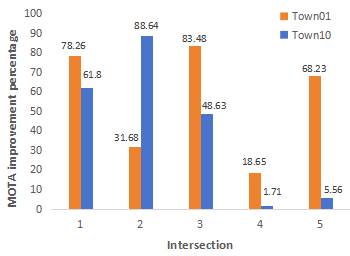
\includegraphics[width=\linewidth]{picture/picture4.png} 
	\caption{Comparison of \(RMOTA\) improvement (\%) after hyperparameter optimization on Town01 and Town10. The results demonstrate the effectiveness of the optimization strategies used in different scenarios.} 
	\label{fig:4} 
\end{figure}

\subsection{Limitations and Future Directions}

\textbf{Problems Encountered in The Experiment.}
During our experiments, we encountered the following issues:  
1.When matching trajectories across multiple intersections, images of vehicles corresponding to each trajectory are needed to extract re-identification appearance features. 
Acquiring these images is difficult, and the methods used can affect accuracy.  
2.When matching trajectories, it is necessary to associate trajectories from all intersections. 
However, due to ID switching, the trajectory of the same vehicle at a single intersection may be fragmented, making integration complex. 
If only one trajectory is selected as the current intersection's trajectory for a vehicle, issues arise when the same vehicle returns to the intersection.

\textbf{Shortcomings of Current Research.}
Although our experiments have achieved some success, there are still some limitations. 
For example, the detection accuracy of PointPillars is not high, resulting in suboptimal tracking performance. 
Additionally, false detections may occur when acquiring images of vehicles corresponding to current trajectories, potentially leading to trajectory matching errors.

\textbf{Vision of The Future.}
Our experiments were conducted under offline conditions, meaning they lacked real-time capabilities. 
In future work, we aim to transition these experiments to an online framework to achieve high real-time performance, thereby enhancing their experimental value.


\section{Conclusion}

Through a series of experiments, we have demonstrated the application value of UVDT in intelligent transportation. 
Digital twin technology can not only accurately replicate real-world traffic scenarios but also effectively predict future traffic conditions. 
Multi-target tracking and the inference of unknown trajectories serve as strong evidence of this capability. 
This holds significant value for the development of future cities.
We hope that new large-scale datasets will be introduced in the future to further enhance the effectiveness of digital twins.


\bibliographystyle{IEEEtran}
\bibliography{reference}

\end{document}


